%% abtex2-modelo-projeto-pesquisa.tex, v-1 PFC 1 2016
%% Copyright 2012-2015 by abnTeX2 group at http://www.abntex.net.br/ 
%%
%% This work consists of the files abntex2-modelo-projeto-pesquisa.tex
%% and abntex2-modelo-references.bib
%%
% ------------------------------------------------------------------------
% ------------------------------------------------------------------------
% abnTeX2: Modelo de Projeto de pesquisa em conformidade com 
% ABNT NBR 15287:2011 Informação e documentação - Projeto de pesquisa -
% Apresentação 
% ------------------------------------------------------------------------ 
% ------------------------------------------------------------------------

\documentclass[
	% -- opções da classe memoir --
	12pt,				% tamanho da fonte
	openright,			% capítulos começam em pág ímpar (insere página vazia caso preciso)
	oneside,
    %twoside,			% para impressão em verso e anverso. Oposto a oneside
	a4paper,			% tamanho do papel. 
	% -- opções da classe abntex2 --
	%chapter=TITLE,		% títulos de capítulos convertidos em letras maiúsculas
	%section=TITLE,		% títulos de seções convertidos em letras maiúsculas
	%subsection=TITLE,	% títulos de subseções convertidos em letras maiúsculas
	%subsubsection=TITLE,% títulos de subsubseções convertidos em letras maiúsculas
	% -- opções do pacote babel --
	english,			% idioma adicional para hifenização
	french,				% idioma adicional para hifenização
	spanish,			% idioma adicional para hifenização
	brazil,				% o último idioma é o principal do documento
	]{abntex2}

% ---
% PACOTES
% ---

% ---
% Pacotes fundamentais 
% ---
\usepackage{lmodern}			% Usa a fonte Latin Modern
\usepackage[T1]{fontenc}		% Selecao de codigos de fonte.
\usepackage[utf8]{inputenc}		% Codificacao do documento (conversão automática dos acentos)
\usepackage{indentfirst}		% Indenta o primeiro parágrafo de cada seção.
\usepackage{color}				% Controle das cores
\usepackage{graphicx}			% Inclusão de gráficos
\usepackage{microtype} 			% para melhorias de justificação
\usepackage{verbatim}           % comentar em bloco
\usepackage{longtable}

% ---

% ---
% Pacotes adicionais, usados apenas no âmbito do Modelo Canônico do abnteX2
% ---
\usepackage{lipsum}				% para geração de dummy text
% ---

% ---
% Pacotes de citações
% ---
\usepackage[brazilian,hyperpageref]{backref}	 % Paginas com as citações na bibl
\usepackage[alf]{abntex2cite}	% Citações padrão ABNT

% --- 
% CONFIGURAÇÕES DE PACOTES
% --- 

% ---
% Configurações do pacote backref
% Usado sem a opção hyperpageref de backref
\renewcommand{\backrefpagesname}{Citado na(s) página(s):~}
% Texto padrão antes do número das páginas
\renewcommand{\backref}{}
% Define os textos da citação
\renewcommand*{\backrefalt}[4]{
	\ifcase #1 %
		Nenhuma citação no texto.%
	\or
		Citado na página #2.%
	\else
		Citado #1 vezes nas páginas #2.%
	\fi}%
% ---

% ---
% Informações de dados para CAPA e FOLHA DE ROSTO
% ---
\titulo{Uso de Redes Neurais Artificiais na Predição do Risco de Reprovação de Alunos na Educação em Computação}
\autor{Lucas Rodrigues Costa} % do Curso de Ciências da Computação}
\local{Jataí-GO}
\data{2019}
\tipotrabalho{Projeto de Pesquisa (Graduação)}
% O preambulo deve conter o tipo do trabalho, o objetivo, 
% o nome da instituição e a área de concentração 
\preambulo{Projeto de Pesquisa apresentado ao curso de Bacharelado em Ciências da Computação, como requisito para obtenção do grau final na disciplina de Projeto Final de Curso 1.}

\orientador {Prof. Me. Esdras Lins Bispo Jr.}

\instituicao{Universidade Federal de Goiás - Regional Jataí}

% ---

% ---
% Configurações de aparência do PDF final

% alterando o aspecto da cor azul
\definecolor{blue}{RGB}{41,5,195}

% informações do PDF
\makeatletter
\hypersetup{
     	%pagebackref=true,
		pdftitle={\@title}, 
		pdfauthor={\@author},
    	pdfsubject={\imprimirpreambulo},
	    pdfcreator={LaTeX with abnTeX2},
		pdfkeywords={abnt}{latex}{abntex}{abntex2}{projeto de pesquisa}, 
		colorlinks=true,       		% false: boxed links; true: colored links
    	linkcolor=blue,          	% color of internal links
    	citecolor=blue,        		% color of links to bibliography
    	filecolor=magenta,      		% color of file links
		urlcolor=blue,
		bookmarksdepth=4
}
\makeatother
% --- 

% --- 
% Espaçamentos entre linhas e parágrafos 
% --- 

% O tamanho do parágrafo é dado por:
\setlength{\parindent}{1.3cm}

% Controle do espaçamento entre um parágrafo e outro:
\setlength{\parskip}{0.2cm}  % tente também \onelineskip

% ---
% compila o indice
% ---
\makeindex
% ---

% ----
% Início do documento
% ----
\begin{document}

% Seleciona o idioma do documento (conforme pacotes do babel)
%\selectlanguage{english}
\selectlanguage{brazil}

% Retira espaço extra obsoleto entre as frases.
\frenchspacing 

% ----------------------------------------------------------
% ELEMENTOS PRÉ-TEXTUAIS
% ----------------------------------------------------------
% \pretextual

% ---
% Capa
% ---
\imprimircapa
% ---

% ---
% Folha de rosto
% ---
\imprimirfolhaderosto
% ---

% ---
% NOTA DA ABNT NBR 15287:2011, p. 4:
%  ``Se exigido pela entidade, apresentar os dados curriculares do autor em
%     folha ou página distinta após a folha de rosto.''
% ---

% ---
% inserir lista de ilustrações
% ---
\pdfbookmark[0]{\listfigurename}{lof}
\listoffigures*
\cleardoublepage
% ---

% ---
% inserir lista de tabelas
% ---
\pdfbookmark[0]{\listtablename}{lot}
\listoftables*
\cleardoublepage
% ---

% ---
% inserir lista de abreviaturas e siglas
% ---
\begin{siglas}
  %\item[ABNT] Associação Brasileira de Normas Técnicas
  %\item[abnTeX] ABsurdas Normas para TeX
  \item[ARL - Análise de Regressão Linear]
  \item[EaD - Ensino à Distância]
  \item[GBL - \textit{Games-based Learning}]
  \item[IpC - Instrução pelos Colegas]
  \item[IA - Inteligência Artificial]
  \item[INEP - Instituto Nacional de Estudos e Pesquisas Educacionais Anísio Teixeira]
  \item[MDE - Mineração de Dados Educacionais]
  \item[MEC - Ministério da Educação]
  \item[PEC - Pesquisa em Educação de Computação]
  \item[PI - \textit{Peer Instruction}]
  \item[RNA - Redes Neurais Artificiais]
  \item[SIGCSE - \textit{Special Interest Group onComputer Science Education}]
  \item[STI - Superintendência de Tecnologia da Informação]
  \item[UFG - Universidade Federal de Goiás]
  \item[UFPB - Universidade Federal da Paraíba]
  \item[WEI - Workshop sobre Educação em Computação]
  \item[WEKA - \textit{Waikato Environment for Knowledge Analysis}]


\end{siglas}
% ---

\begin{comment}{
% ---
% inserir lista de símbolos
% ---
\begin{simbolos}
  \item[$ \Gamma $] Letra grega Gama
  \item[$ \Lambda $] Lambda
  \item[$ \zeta $] Letra grega minúscula zeta
  \item[$ \in $] Pertence
\end{simbolos}
% ---
}\end{comment}

% ---
% inserir o sumario
% ---
\pdfbookmark[0]{\contentsname}{toc}
\tableofcontents*
\cleardoublepage
% ---


% ----------------------------------------------------------
% ELEMENTOS TEXTUAIS
% ----------------------------------------------------------
\textual

% ----------------------------------------------------------
% Introdução
% ----------------------------------------------------------
\chapter*[Introdução]{Introdução}
\addcontentsline{toc}{chapter}{Introdução}

\begin{comment}{
%==========================================================================================
{\color{red}[MODELO]
A INTRODUÇÃO é apresentada em forma de um texto “corrido”, ou seja, de uma única redação em que deverão ser apresentados os elementos: tema (objeto de estudo, problema e área/sub-área); objetivos (geral e específicos) e justificativas.

Contextualiza-se o tema segundo o Marco Teórico/Estado da Arte que sustentará o desenvolvimento da pesquisa. Há que se esclarecer os limites para o seu desenvolvimento, a JUSTIFICATIVA da investigação por meio de uma REVISÃO BIBLIOGRÁFICA, em que se faz referência a estudos e pesquisas já realizados sobre o assunto em questão. O TEMA da pesquisa define o objeto de estudo a ser tratado. Pode equivaler ou não ao título do projeto ou da pesquisa. Deve ter um significado preciso. Já o PROBLEMA deve ser ainda mais específico e detalhado que o objeto de estudo. O problema também deve ser pautado em um levantamento bibliográfico. O problema, formulado como pergunta, deve ser associado ao marco teórico da investigação a ser feita e as demandas institucionais e sociais. Além disso, deve ser completo, ou seja, conter as variáveis necessárias e esclarecedoras da investigação. 
A revisão bibliográfica, para justificar a pesquisa, pode ser feita, optando-se por um dos seguintes argumentos:
\begin{enumerate}
\item o pesquisador demonstra a análise incompleta ou insuficiente acerca do objeto de estudo;
\item por meio da literatura selecionada, o estudioso demonstra contradições entre os autores em relação ao problema enunciado;
\item o estudioso deseja colocar em xeque as conclusões encontradas sobre o objeto de estudo;
\item o pesquisador necessita retestar os resultados já obtidos em outras investigações.
\item a área carece de inovações, adequações, melhorias ou contribuições acerca de uma tema.
\item a área pode ser solução para melhoria ou resolução de problemas de outras áreas afins ou não.
\end{enumerate}

Os OBJETIVOS são as metas conceituais a serem alcançadas com a realização do trabalho, por meio de verbos no infinitivo, como: demonstrar, identificar, observar, analisar, comparar. A melhor forma de destacá-los é dividi-los em geral / específicos. O GERAL deve se referir ao produto que se deseja obter com a investigação. 

Já OBJETIVOS ESPECÍFICOS (devem conter, no mínimo, três) possuem natureza operacional, isto é, referem-se a procedimentos que deverão ser cumpridos para que o objetivo geral seja atingido, confirmando ou não a hipótese enunciada.

É importante lembrar ao definir os objetivos específicos que os mesmos devem estar coerentes com a metodologia do trabalho (passos necessários para atingir os objetivos) e com o cronograma (tempo/prazo de execução do trabalho).
Para enriquecer a seção de Objetivos (geral e específicos) é salutar apresentar estratégias para atingir os objetivos e quantificar metas a serem alcançadas.
	
    A HIPÓTESE é a tentativa de explicação ou solução do problema enunciado, expressa na forma de sentença afirmativa. Deve também estar de acordo com o Estado da Arte/Marco Teórico definido. Trata-se de um ato criativo. Deve possuir clareza conceitual, referir-se a conceitos passíveis de verificação (empírica). A \autoref{metodo_cient} ilustra quais são as fases de uma pesquisa.

\begin{figure}[!htb]
    \centering
    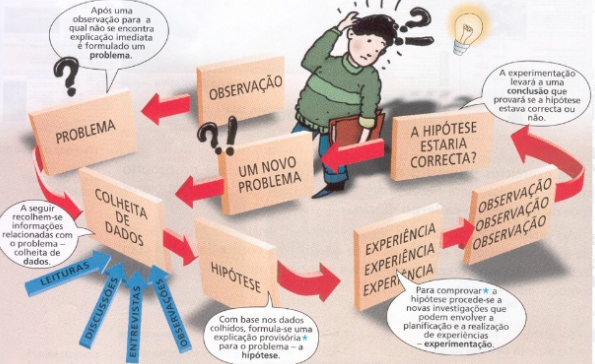
\includegraphics[scale=0.70]{metodo.png}
    \caption{Fases de uma pesquisa}
    \label{metodo_cient}
\end{figure}

Uma lista completa das normas
observadas pelo \abnTeX\ é apresentada em \citeonline{abntex2classe}.



Este documento deve ser utilizado como complemento dos manuais do \abnTeX\ 
\cite{abntex2classe,abntex2cite,abntex2cite-alf}. Consulte \citeonline{abntex2modelo} para obter
exemplos e informações adicionais de uso de \abnTeX\ e de \LaTeX. }
}
%===========================================================================================
\end{comment}

%Objeto de estudo
%Problema
%Área
%Objetivos
    % - Geral
    % - Específico
%Justificativa

%Ideias principais, da maior pra menor

% 1 - Afirmação geral sobre a área: Educação de computação
% 2 - Problema da área: Avaliação, identificação prévia de alunos em situação de risco
% 3 - Como os autores da área vem resolvendo esse problema
    % 3.1 - Para tentar resolver esse problema, esse autor fez isso.
    % 3.2 - Para tentar resolver, esse autor fez isso.
    % 3.3 - Para...
% É possível que essas soluções apresentem lacunas. Cewrtamente, usar no Brasil
% A proposta do meu trabalho é: Atacar essa lacuna diante do que já existe

% 1

A Educação em Computação é uma área emergente e amplamente discutida pela comunidade acadêmica internacional \cite{fincher2005mapping}. No contexto brasileiro, o Workshop sobre Educação em Computação (WEI) tem sido um dos principais fóruns para esta discussão. O SIGCSE (\textit{Special Interest Group on Computer Science Education}) \textit{Technical Symposium} é um dos maiores eventos, em âmbito internacional, na área. Pode-se definir, como um dos objetivos principais da PEC (Pesquisa em Educação de Computação), o aperfeiçoamento do processo de ensino e aprendizagem da Computação como ciência \cite{holmboe2001research}

%Problema
Muitos alunos ingressantes em Computação apresentam dificuldades na aprendizagem, assim como em outras áreas de exatas \cite{blando2015dificuldades}. Em virtude destas dificuldades, alguns alunos não alcançam um desempenho satisfatório e reprovam em alguma disciplina. Estas reprovações podem ter, dentre outros fatores, forte influência em uma eventual evasão \cite{evasaoMatheus2014}. Segundo dados do Censo da Educação Superior de 2017 \cite{Inep2017}, publicado pelo Instituto Nacional de Estudos e Pesquisas Educacionais Anísio Teixeira (INEP) do Ministério da Educação (MEC), a taxa de evasão do Bacharelado em Ciência da Computação, nas universidades públicas e privadas de todo o Brasil, alcançou cerca de 60,2\%, enquanto a taxa geral - média dentre todos os cursos - ficou em torno dos 26\%.

Desta forma, um dos problemas na Educação em Computação é a investigação de meios mais eficazes de realizar a avaliação de aprendizagem dos alunos. Um destes interesses consiste em identificar previamente aqueles alunos que apresentam maior dificuldade na disciplina e, assim, têm maior risco de reprovação.\cite{martins2012assistente}, esses alunos que se encontram em situação de risco de reprovação são integrantes do chamado ``grupo de risco''\footnote[1]{Alunos em risco: Os alunos em situação de risco são aqueles que estão propensos a não concluir um curso, seja por insuficiência de presença ou de desempenho. \cite{da2014alunos}}. Diversos autores propõem diferentes métodos para solucionar este problema. Alguns destes autores abordam modelos preditivos em relação à situação dos alunos.
%Justificativa
%Muitas vezes os ingressantes não conseguem acompanhar o fluxo de estudos, têm baixo desempenho e assim acabam evadindo ou reprovando nas matérias introdutórias do curso.
%Um dos pontos está no interesse 
 %{\color{red}[TERMINAR]}

%Alguns autores propuseram métodos para solucionar esse problema. Podemos citar alguns autores e seus trabalhos, que abordaram modelos preditivos quanto a situação dos alunos.



%Lightweight, Early Identification of At-Risk CS1 Students
\citeonline{liao2016lightweight} utilizaram o modelo de \textbf{ARL (Análise de Regressão Linear)}, para fazer a análise dos dados gerados através do uso do IpC (Instrução pelos Colegas)\footnote[2]{Do inglês, \textit{Peer Instruction} (PI)}, juntamente com o \textit{Clicker}, pelos alunos, para tentar identificar os que estariam com tendência a baixo desempenho na disciplina, baseado nas respostas dadas nas 3 primeiras semanas de aulas. O modelo proposto alcançou, aproximadamente, 70\% de acurácia na identificação de alunos com risco de reprovação, com 17\% dos alunos reprovados sendo erroneamente classificados - ``falsos negativos''\footnote[3]{``Falsos negativos'': Quando os alunos são previamente classificados como não-integrantes do ``Grupo de risco'', mas que, ao final da disciplina, acabaram reprovando}.

%Modelo de Regressão Linear aplicado à previsão de desempenho de estudantes em ambiente de aprendizagem
\textbf{ARL} também foi usada no trabalho de \citeonline{rodrigues2013modelo}, onde investigou-se a viabilidade da aplicação de técnicas de modelagem de regressão linear para realizar inferências relativas ao desempenho de estudantes. Os resultados obtidos com o experimento confirmam que é viável, podendo afirmar que é possível estimar o resultado acadêmico de alunos baseado na quantidade de interações em ferramentas do tipo fórum de discussão. 

%Importance of early performance in CS1: two conflicting assessment stories
\citeonline{porter2014importance} usam os dados coletados durante o uso do IpC, além dos dados de provas, para explorar as relações entre as avaliações e o desempenho em sala de aula no final do prazo. Para examinar a relação entre as notas dos alunos em avaliações diferentes, foi utilizada a \textbf{Correlação de Pearson}.

%Automatically Classifying Students in Need of Support by Detecting Changes in Programming Behaviour
\citeonline{estey2017automatically} propuseram um método preditor que detecta, com 81\% de precisão, os estudantes em situação de risco de reprovação na disciplina de programação. O estudo foi desenhado para avaliar a aprendizagem do aluno através da detecção de \textbf{mudanças no comportamento} de programação ao longo do tempo. 

 Uma outra proposta é o uso do \textbf{modelo PreSS} que usa fatores comparativos - como a eficiência de programação, a habilidade matemática  e as horas dedicadas em exercícios - para auxiliar a identificação do alunos em risco de reprovação \cite{quille2018}. Existem até ferramentas capazes de realizarem capturas de telas, que exibem código-fonte, para auxiliar na identificação das dificuldades apresentadas pelos alunos usando \textbf{aprendizado de máquina} \cite{ahadi2016early}.
 
%Objetivos Geral/Específico
O objetivo geral deste trabalho é prever o desempenho acadêmico, na Educação de Computação, dos alunos --- no contexto brasileiro --- ainda no inicio da disciplina, identificando os que estejam no grupo de risco, possibilitando ao professor intervir. Este projeto de pesquisa tem como objetivos específicos: a implementação do projeto de Rede Neural Artificial, o treinamento e a validação desta e a análise dos resultados através de um estudo de caso no sudoeste goiano, coletando dados com o uso da plataforma "Kahoot!".

%propôr um modelo de Rede Neural Artificial, como método preditivo de desempenho acadêmico, além de suprir a falta de relatos de casos no Brasil, apresentando um estudo de caso no sudoeste goiano, coletando dados na disciplina, durante o uso da plataforma de Aprendizagem Baseado em Jogos, ``Kahoot!'', como forma de avaliação formativa.
%na disciplina de Interface Humano-Computador, no curso de Ciência da Computação da Universidade Federal de Goiás - Regional Jataí/Universidade Federal de Jataí.

%Objeto de estudo
%Esta pesquisa tem como objeto de estudo a Avaliação da Aprendizagem de Ciência da Computação. e o problema de avaliação e identificação preditiva do desempenho acadêmico de alunos, com base os dados coletados dos alunos em avaliações formativas no inicio da disciplina.

% ----------------------------------------------------------
% Elementos Textuais
% ----------------------------------------------------------
\chapter{Referencial Teórico}
Para melhor compreensão do texto, é importante estabelecer as definições de alguns conceitos que serão adotados neste projeto de pesquisa. 

\begin{comment}{
{\color{red}[MODELO]
\index{elementos textuais} O Referencial Teórico é um seção dos elementos textuais. A norma ABNT NBR 15287:2011, p. 5, apresenta a
seguinte orientação quanto aos elementos textuais:

\begin{citacao}
O texto deve ser constituído de uma parte introdutória, na qual devem ser
expostos o tema do projeto, o problema a ser abordado, a(s) hipótese(s),
quando couber(em), bem como o(s) objetivo(s) a ser(em) atingido(s) e a(s)
justificativa(s). É necessário que sejam indicados o referencial teórico que
o embasa, a metodologia a ser utilizada, assim como os recursos e o cronograma
necessários à sua consecução.\citeonline{abntex2classe}
\end{citacao}, ,

Deve-se apresentar a fundamentação teórica que orientará o estudo. Recomenda-se situar a grande área, subárea e objeto de estudo. Se for necessário pode ser feito um resgate histórico para demonstrar a evolução da área. Faz-se necessário relatar o momento vivido pela área (Marco Teórico - Estado da Arte) geralmente intitulado de Trabalhos Relacionados.

O Referencial Teórico é considerado como um elemento de controle de toda a pesquisa, desde a problematização inicial. O pesquisador irá interpretar seu objeto de estudo de acordo com a concepção teórica de uma ou toda a obra de um autor ou de um objeto ou produto ou de um conjunto de autores (esta condução varia de acordo com cada área de conhecimento). Todas as etapas do projeto são definidas conforme esta escolha. Apresenta-se de modo aprofundado, respondendo quais os princípios, categorias, conceitos ou teorias fundamentam a pesquisa. Deve estar de acordo com o tema formulado e o raciocínio desenvolvido nas fases anteriores. 

}}\end{comment}

\section{Educação de Computação}
\label{sec:EC}

Educação de computação é o resultado da fusão de, a princípio --- Outras também estão envolvidas, como: Psicologia, engenharias, tecnologia, entre outras ---, duas disciplinas: Educação e Computação. 

Educação é um processo que visa ao desenvolvimento físico, intelectual e moral do ser humano, através da aplicação de métodos próprios, com intuito de assegurar-lhe a integraçãoo social e formal da cidadania \cite{weiszflog1999michaelis}. Ciência da Computação é o estudo sistemático de algoritmo e estrutura de dados, i.e., o estudo do seu formalismo, desenvolvimento e aplicações. \cite{gibbs1986model}

O objetivo principal da pesquisa em Educação de Computação é o aperfeiçoamento do processo de ensino e apredizagem da Computação como ciência. \cite{holmboe2001research}

\citeonline{fincher2005mapping} identificam dez grandes áreas de interesse para pesquisadores em Educação de Computação. As dez áreas são: a compreensão do aluno, sistemas de animação/visualização/simulação, métodos de ensino, avaliação, tecnologia educacional, a transferência de prática profissional em sala de aula, a incorporação de um novo desenvolvimento e novas tecnologias na sala de aula, transferindo para o ensino à distância (“EaD” ou “\textit{e-learning}”), recrutamento e retenção de alunos, a construção da disciplina em à distância (“EaD” ou “\textit{e-learning}”), e finalmente, a construção da disciplina em si. 

%Artigos ============================
%{\color{red}LER}\cite{da2014metodos}

\section{Avaliação}
\label{sec:AVA}
A avaliação é uma área ampla, que pode ser dividida em termos de tipos de avaliação, validade da avaliação e classificação automatizada. \cite{fincher2005mapping}

Segundo \citeonline{libaneo1994didatica}, avaliação pode ser definida como um componente do processo de ensino que visa, através da verificação e qualificação dos resultados obtidos, determinar a correspondência  deste com os objetivos propostos e, daí, orientar a tomada de decisões em relação às atividades didáticas subsequentes.

Outra definição foi dada por \citeonline{domingos1981forma}, onde a avaliação pode ser entendida como um processo sistemático de determinar a extensão em que os objetivos educacionais foram alcançados pelos alunos. O que se avalia são as metas de aprendizagem definidas e para as quais se caminhou durante todo um processo de aprendizagem levado a cabo pelo professor e pelo aluno

A avaliação da aprendizagem possibilita a tomada de decisão e a melhoria da qualidade de ensino, informando as ações em desenvolvimento e a necessidade de regulações constantes. \cite{kraemer2005avaliaccao}

Para \citeonline{datrino2015avaliaccao}, avaliação vista como uma etapa da aprendizagem passa a ser utilizada como um processo, isto é, na formação e construção do conhecimento levando a uma reflexão sobre as ações, gestos e pensamentos. Os processos formativos precisam ser avaliados em sua forma, efeito, método e evolução dos educandos.

Os métodos avaliativos são de suma importância no processo de ensino-aprendizagem. Diversos autores demonstram os benefícios resultantes de uma boa avaliação durante as aprendizagens e conhecimentos adquiridos pelos discentes. Porém, é preciso que sejam escolhidos e aplicados no cotidiano do aluno de forma a conduzi-lo à aprendizagem, obtendo assim resultados satisfatórios a partir de sua avaliação e evitando análises errôneas e estresse por parte dos educadores e educandos. \cite{da2014alunos}

Segundo \citeonline{libaneo1994didatica}, o entendimento correto da avaliação consiste em considerar a relação mútua entre os aspectos quantitativos e qualitativos. A avaliação não pode ser vista apenas como ``medida'', mas também não pode ser baseada na subjetividade de professores e alunos.

\citeonline{bloom1983manual} classificaram a avaliação em três tipos, sendo eles:
avaliação diagnóstica; avaliação formativa e avaliação somativa.

\subsection{Avaliação diagnóstica}
\label{sec:AvaDiag}
Conhecer o aluno, seus gostos, seus hábitos e suas preferências, é o princípio base da avaliação diagnóstica. Dessa forma, assegura-se que o aluno esteja na turma correta e que o curso encontrese no nível adequado a ele. Nesta avaliação busca-se conhecer ideias e conhecimentos prévios do aluno \cite{masetto1994didatica}.

Para \citeonline{bloom1983manual}, avaliação diagnóstica visa verificar a existência, ou ausência, de
habilidades e conhecimentos pré‐estabelecidos, esta é uma ação que inicia o
processo avaliativo e verifica se os alunos dominam os pré‐requisitos necessários
para novas aprendizagens.

Segundo \citeonline{haydtavaliaccao}, a partir de uma avaliação diagnóstica o docente constata se os seus alunos estão ou não preparados, se possuem domínio de pré–requisitos para adquirir novos conhecimentos. Portanto, a avaliação diagnóstica permite que o professor conheça seu aluno por um mecanismo de triagem e calibração

\subsection{Avaliação somativa}
\label{sec:AvaSom}
Avaliação somativa é uma decisão que leva em conta a soma de um ou mais resultados e pode ser baseada numa só prova final \cite{e2004aprender}.

De acordo com \citeonline{haydtavaliaccao}, esse tipo de avaliação tem por princípio classificar os resultados de aprendizagem alcançados pelos alunos de acordo com os níveis de aproveitamento estabelecidos, adotando assim uma função classificatória.

A avaliação somativa pretende ajuizar o progresso realizado pelo aluno, no final de uma unidade de aprendizagem, no sentido de aferir resultados já recolhidos por avaliações do tipo formativo e obter indicadores que permitam aperfeiçoar o processo de ensino \cite{kraemer2005avaliaccao}.

\subsection{Avaliação formativa}
\label{sec:AvaFor}
A idéia de avaliação formativa é sistematizar o funcionamento, levando o professor a
observar mais metodicamente os alunos, a compreender melhor seus funcionamentos, de modo
a ajustar de maneira mais sistemática e individualizada suas intervenções pedagógicas e as
situações didáticas que propõe, tudo isso na expectativa de otimizar a aprendizagem. A
avaliação formativa está portanto centrada essencialmente, direta e imediatamente, sobre a gestão das aprendizagens dos alunos (pelo professor e pelos interessados). Essa concepção se situa abertamente na perspectiva de uma regulação intencional, cuja intenção seria determinar ao mesmo tempo o caminho já percorrido por cada um e aquele que resta a percorrer com vistas a intervir para otimizar os processos de aprendizagem em curso. \cite{perrenoud1999avaliaccao}

A avaliação formativa responde a uma concepção do ensino que considera que aprender é um longo processo, por meio do qual o aluno vai reestruturando seu conhecimento a partir das atividades que executa. Esse tipo de avaliação tem como finalidade fundamental a função ajustadora do processo de ensino-aprendizagem para possibilitar que os meios de formação respondam as características dos alunos. Pretende-se detectar os pontos fracos da aprendizagem, mais do que determinar quais os resultados obtidos com essa aprendizagem. \cite{jorba2003funccao}

\section{Inteligência Artificial}
\label{sec:IA}
A IA (Inteligência Artificial) é uma das ciências mais recentes. O trabalho começou logo após Segunda Guerra Mundial, tendo este nome cunhado em 1956. \cite{russell2004inteligencia}

Segundo \citeonline{bellman1978introduction}, a IA é a automatização de atividades que podem ser associadas ao pensamento humano, atividades como a tomada de decisões, a resolução de problemas, o aprenddizado, entre outros.

Várias disciplinas contribuíram com ideias, pontos de vista e técnicas para a IA. Dentre elas estão: Filosofia, Matemática, Economia, Neurociência, Psicologia, Engenharia de Computadores, Teoria de Controle e Cibernética, Linguística, entre outras. \cite{russell2004inteligencia}

A IA abrange uma enorme variedade de subcampos, desde áreas de uso geral, como aprendizado e percepção, até tarefas específicas como diagnóstico de doenças, por exemplo. A IA sistematiza e automatiza tarefas intelectuais e, portanto, é potencialmente relevante para qualquer esfera da atividade intelectual humana. \cite{russell2004inteligencia}

De acordo com \citeonline{sage1990concise}, o objetivo da IA é o desenvolvimento de paradigmas ou algoritmos que requeiram máquinas parar realizar tarefas cognitivas, para as quais os humanos são atualmente melhores. Um sistema de IA tem três componentes fundamentais: representação, raciocínio e aprendizagem.

Aprendizado de Máquina é uma área da IA cujo objetivo é o desenvolvimento de técnicas computacionais sobre o aprendizado bem como a construção de sistemas capazes de adquirir conhecimento de forma automática. Um sistema de aprendizado é um programa de computador que toma decisões baseado em experiências acumuladas através da solução bem sucedida de problemas anteriores. Os diversos sistemas de aprendizado de máquina possuem características particulares e comuns que possibilitam sua classificação quanto à linguagem de descrição, modo, paradigma e forma de aprendizado utilizado \cite{monard2003sistemas}.
Umas das técnicas de aprendizado de máquina são as Redes Neurais Artificiais.

%\subsection{Aprendizado de Máquina}

\subsection{Redes Neurais Artificiais}
\label{sec:RNA}
Um neurônio é uma célula no cérebro cuja a principal função é coletar, processar e disseminar sinais elétricos. Uma parte do trabalho inicial da IA teve como objettico criar \textbf{Redes Neurais Artificiais} (RNA). Estas são funções não-lineares complexas com muitos parâmetros. \cite{russell2004inteligencia}

Segundo \citeonline{haykin2001redes}, uma rede neural é um processador maciçamente paralelamente distribuído constituído de unidades de processamento simples, que têm a propensão natural para armazenar conhecimento experimental e torná-lo disponível para o uso. Ela se assemelha ao cérebro em dois aspectos: Conhecimento adquirido pela rede, através de um processo de aprendizagem. Forças de conexão entre neurônios, conhecidos como pesos sinápticos, usados para armazenar o conhecimento adquirido.

\citeonline{haykin2001redes} descreveu ainda que a arquitetura de uma rede neural restringe o tipo de problema no qual a rede poderá ser utilizada, e é definida pelo número de camadas (camada única ou múltiplas camadas), pelo número de nós em cada camada, pelo tipo de conexão entre os nós (\textit{feedforward} ou \textit{feedback}) e por sua topologia.

\section{Aprendizagem Baseada em jogos - \textit{Games-based Learning}}
\label{sec:GBL}

Aprendizagem Baseada em jogos, ou GBL (pela sigla em inglês de \textit{Games-based Learning}), foi definida por alguns autores. Segundo \citeonline{tang2009introduction}, GBL faz referência a uma abordagem de aprendizagem inovadora derivada do uso de jogos de computador que tem valor educacional ou diferentes tipos de aplicação de software que usam jogos computacionais para ensino e educação. GBL's têm como finalidade o apoio à aprendizagem, a avaliação e análise de alunos e melhoria do ensino.

A aprendizagem baseada em jogos surge como uma alternativa de ensino que se adapta às características da pedagogia moderna na qual o estudante é um ator ativo \cite{monsalve2014aprendizagem}.

Com a aprendizagem baseada em jogos, se pretende equilibrar entretenimento e difusão do conhecimento, motivando os estudantes a aprender enquanto jogam \cite{monsalve2011teaching}.

\citeonline{Souza:2017:GLB:3103028.3103054} definiram \textit{GBL} como o ato de aplicar jogos com o propósito de aprender habilidades e conceitos específicos, geralmente nomeado como “jogos sérios” (jogos com fins), entretenimento educativo\footnote{Do termo, em inglês, “\textit{Edutainment}”, que seria a união de educação (\textit{Education}) e entreterimento (\textit{entertainment})} ou jogos educativos.

\citeonline{von2009game} definiram GBL como uma abordagem lida com aplicativos de jogos que definiram resultados de aprendizagem.

Algumas plataformas de GBL foram utilizadas por autores no processo de ensino-aprendizagem. Um destes foi o de \citeonline{lot2016game}, onde abordaram o uso de GBL como avaliação formativa, com a plataforma \textbf{Zoondle}. Outras plataformas de GBL usadas foram a \textbf{EducaCross}, no trabalho de \citeonline{reis2016experiencia}, a \textbf{Timemesh}, no trabalho de \citeonline{}{baptista2013timemesh} e, provavelmente o mais popular, \textbf{Kahoot!}, que será usado neste projeto de pesquisa.

\subsection{Kahoot!}
\label{sec:Kahoot!}
Kahoot! é uma plataforma de aprendizado baseada em jogos, usada como tecnologia educacional em escolas, universidades e outras instituições de ensino. Kahoot! foi fundada por Johan Brand, Jamie Brooker e MortenVersvik em um projeto conjunto com a Universidade Norueguesa de tecnologia e ciência \cite{kahoot2018}

Seus jogos de aprendizado, ``Kahoots'', são \textit{quizzes}, perguntas de múltipla escolha, que permitem a criação de usuários e podem ser acessados por meio de um navegador da Web, telefone ou pelo aplicativo.

Kahoot! foi projetado para a aprendizagem social, com os alunos reunidos em torno de uma tela comum, como um quadro interativo, projetor ou um monitor de computador. O site também pode ser usado por meio de ferramentas de compartilhamento de tela, como Skype ou Google hangouts. Kahoot! pode ser usado para revisar o conhecimento dos alunos, para avaliação formativa \cite{kahootFormative}, ou como uma pausa com as atividades tradicionais em sala de aula. 

A jogabilidade é simples; todos os jogadores se conectam usando um PIN de jogo gerado na tela comum e usam um dispositivo para responder a perguntas criadas pelo professor. As questões podem ter pontuações atribuídas, em relação ao acerto e ao tempo para resposta. Os pontos aparecem no placar depois de cada pergunta.

Alguns trabalhos relataram os resultados encontrados ao utilizar o Kahoot! no processo de ensino. Um destes foi realizado por \citeonline{diniz2018kahoot}, que usou a ferramenta com alguns alunos de Ciência da Computação, obtendo resultados satisfatórios quanto a aceitação da ferramenta no contexto educacional.

\begin{comment}
%Artigos complementares
{\color{red}LER}
    
    \cite{chaiyo2017effect}\\
    \cite{tobias2014game}\\
    \cite{wang2015wear}\\
    \cite{connolly2012systematic}\\
    \cite{backlund2013educational}
\end{comment}
    
 Considerando que alguns fatores sociais e geográficos podem afetar a aplicação e a eficiência do uso desta ferramenta, faz-se necessário avaliá-la no contexto dos estudantes brasileiros.
 
 No trabalho de \citeonline{petri2016quiz}, o Kahoot! foi utilizado como um \textit{quiz} com perguntas sobre Gerenciamento de Projetos, disponibilizado para alunos dos cursos de Sistemas de
Informação e Ciência da Computação como forma de revisão de conteúdo. Os autores identificaram \textit{feedbacks} positivos nos resultados encontrados. Afirmaram também que o jogo educacional cumpriu com o seu objetivo de aprendizagem por proporcionar a revisão de conhecimentos de forma divertida e motivadora.

Para os autores \citeonline{abidin2017students}, a utilização do Kahoot! foi uma estratégia de motivação para os alunos de uma faculdade de Engenharia Elétrica ao cursarem uma disciplina de programação de computadores. O conteúdo apresentado no \textit{game} era relacionado a disciplina em questão e o objetivo era possibilitar aos alunos uma experiência atrativa para a aprendizagem, pois muitos deles perdiam o entusiamo ao estudarem programação de computadores. O resultado mostrou que a grande maioria dos alunos conseguiu melhorar sua  compreensão sobre a disciplina e também se mostraram mais engajados e motivados ao final do experimento.

Outro trabalho similar foi o realizado por \citeonline{correia2017game}, que apresenta as opiniões de alunos de um programa de formação de professores (licenciatura e mestrado) sobre as vantagens e desvantagens da utilização do Kahoot! em sala de aula. Como vantagens percebidas estão a correção automática das questões e o \textit{feedback} em tempo real para os alunos e professores. Como desvantagens, foram identificados os seguintes fatores: numero limitado de caracteres tanto para o enunciado das questões quanto para as opções de respostas, além do tempo limitado de resposta.

%Artigo WEI
%O principal objetivo do estudo foi identificar percepções acadêmico. Objetivos mais específicos consistiram em verificar a aceitação da mesma com base em algumas perspectivas além de elucidar as vantagens e desvantagens da sua utilização. Os resultados foram bastantes satisfatórios no que diz respeito a aceitação da ferramenta no contexto educacional, pelo seu caráter divertido, interessante e dinâmico os quais remetem a aprendizagem, conforme a percepção dos alunos. Também foi verificado que a sua utilização não causou efeito colateral nas respostas dos participantes.

Kahoot, mantém as mesmas utilidades que outros métodos de resposta rápida; especialmente os \textit{clickers}, mas sem todos os problemas técnicos e logísticos destes. \cite{pintor2014kahoot}

\chapter{Trabalhos Relacionados}
\label{sec:TR}
No decorrer dessa pesquisa foram encontrados alguns trabalhos que propõem métodos para a predição de desempenho acadêmico. Nesta seção, serão apresentados do levantamento bibliográfico feito para encontrar esses trabalhos, os trabalhos correlatos que estão fortemente ligados com este projeto de pesquisa, seguido de breve resumo do que cada autor propôs e obteve como resultado, e uma tabela apresentado as  características de cada um dos trabalhos.

\section{Levantamento Bibliográfico}
\label{sec:Lev}
%Objetivos
\subsection{Objetivo}
\label{sec:Obj}
O objetivo deste levantamento bibliográfico é fazer uma revisão, seleção e organização dos artigos que possam identificar os alunos em situação de risco, analisando os métodos propostos.

%Questões de pesquisa
\subsection{Questões de Pesquisa}
\label{sec:QP}
Para nortear esta levantamento, foram definidas questões que elenquem pontos relevantes a serem estudados.
\begin{itemize}
    \item \textbf{Questão 1}: Quais métodos foram propostos para identificar alunos com risco de reprovação em disciplinas?
    \item \textbf{Questão 2}: Quais os graus de precisão e acurácia alcançados ao utilizar-se destes métodos?
    \item \textbf{Questão 3}: Redes Neurais Artificias foram utilizadas? Se sim, são assertivas na predição de alunos em situação de risco?
    \item \textbf{Questão 4}: Quais são as vantagens de se utilizar Redes Neurais Artificiais para tal?
\end{itemize}

\subsection{Método de pesquisa}
\label{sec:MP}
Nesta seção serão descritos alguns elementos utilizados para o levantamento bibliográfico, de acordo com \citeonline{kitchenham2004procedures}. São estes: o escopo da pesquisa, o idioma considerado, os termos utilizados, a \textit{string} de busca e os critérios de seleção de artigos.


\subsubsection{Máquinas de busca utilizadas}
Para este levantamento bibliográfico, foram escolhidos três das principais máquinas de buscas disponíveis atualmente. Aplicou-se as \textit{Strings} de buscas que serão mais a frente, a fim de identificar potenciais trabalhos correlatos ao tema deste. As máquinas de busca utilizadas para a pesquisa foram:
\begin{itemize}
    \item ACM Digital Library
    \item Google Scholar
    \item IEEE Xplore
\end{itemize}

\subsubsection{Idiomas dos Artigos}
Por se tratarem da língua oficial brasileira e uma das línguas mais faladas, respectivamente, Português e Inglês foram os idiomas escolhido para a pesquisa dos artigos.

\subsection{Palavras-chave e \textit{strings} de busca}

As palavras-chave que compõem a busca são (em português e inglês, respectivamente): 
Educação de Computação, Ensino de Computação, Introdução a Computação, Avaliação, Estimativa, Previsão, Inteligência Artificial, Mineração de Dados, Aprendizado em Profundidade, Redes Neurais Artificiais, RNA, \textit{Computer Education}, \textit{CS1}, \textit{Assessment}, \textit{Prediction}, \textit{Artificial Intelligence}, \textit{Data Mining}, \textit{Clicker}, \textit{Deep Learning}, \textit{Artificial Neural Network}, \textit{ANN}.

A \autoref{string-busca} mostra as \textit{strings} de busca foram geradas a partir da combinação das palavras chave, dividida pelos idiomas estabelecidos.

%\begin{table}[!htb]
\begin{center}
\begin{longtable}{|| p{3cm} || p{10cm} ||}
\caption{String de Busca}
\label{string-busca}
\hline
\textit{\textbf{Português}} & (``Educação de computação'' OR ``ensino de computação'' AND ``Introdução a Computação'' OR ``Avaliação'') AND (``estimativa'' OR ``previsão'' AND ``Inteligência Artificial'' OR ``mineração de dados'' OR ``Aprendizado em Profundidade'' OR ``Redes Neurais Artificiais'' OR ``RNA'')\\
\hline \hline
\textit{\textbf{Inglês}} & \textit{(``Computer Education'' AND ``cs1'' OR ``assessment'') AND (``prediction'' OR ``data mining'' OR ``artificial intelligence'' OR ``deep learning'' OR ``Artificial neural network'' OR ``ANN''))}\\
 \hline \hline
\end{longtable}
\end{center}
%\end{table}

\subsubsection{Critérios de Seleção de Artigos e Procedimentos}
\citeonline{kitchenham2004procedures} diz que devem ser seguidos critérios de inclusão e exclusão para os artigos que são retornados pela \textit{string} de busca. Sendo assim, foram definidos os seguintes critérios:

\subsubsection{Critérios para Inclusão de Artigos}

\begin{enumerate}
    \item Pesquisas as quais tratam sobre utilização de métodos para identificação de alunos em situação de risco de reprovação;
    \item Pesquisas as quais tratam sobre inteligência artificial no contexto educação de computação e no processo de ensino-aprendizagem;
    \item Pesquisas as quais tratam sobre previsão do desempenho acadêmico com uso de aprendizado de máquina.
\end{enumerate}

\subsubsection{Critérios para Exclusão de Artigos}
\begin{enumerate}
    \item Não apresentar necessidade de identificar os alunos em situação de riscos;
    \item Não satisfaçam a nenhum critério de inclusão;
    \item Não apresentar a forma utilizada para coletar dados;
    \item Não apresentou os métodos utilizados para analisar os dados obtidos;
    \item Não foi possível ter acesso a pesquisa completa;
    \item A pesquisa não está disponível na \textit{web};
    \item A pesquisa é publicada apenas como resumo;
    \item Trabalhos que são réplicas ou continuações/evoluções de projetos de pesquisas iniciais, incluindo o trabalho mais completo (Geralmente, o mais recente);
    \item Ter sido publicado em período anterior a 2013.
\end{enumerate}

\subsection{Processo de triagem}
Foi realizada uma primeira triagem, que consistiu na leitura do título, do resumo (\textit{abstract}) e das palavras-chave (\textit{keywords}) dos trabalhos previamente recuperados, aplicando os critérios de inclusão e exclusão e as \textit{Strings} de busca.
A etapa seguinte teve como objetivo realizar a leitura completa e minuciosa dos artigos selecionados na primeira fase. Desta forma, a segunda fase do processo de triagem possibilita fazer uma análise mais apurada dos estudos, identificando e extraindo dados de acordo com os critérios de inclusão e exclusão descritos anteriormente.

\section{Trabalhos Relacionados selecionados}
Após os processos de seleção e triagem, quatro artigos foram considerados fortemente relacionados a este projeto de pesquisa. A seguir, será feito um breve resumo do que foi proposto em cada um deles. Após, será apresentada a \autoref{tab:my-table} com um comparativo de características elencadas para que se faça um paralelo do que já foi proposto por outros autores e o que é alvitrado por este projeto. Por fim, uma breve discussão, destrinchando cada elemento característico dos trabalhos correlatos.

\subsection{Early Identification of Novice Programmers' Challenges in Coding using Machine Learning Techniques}
\label{sec:Early}
Em sua tese de Doutorado, \citeonline{ahadi2016early} usou Mineração de Dados Educacionais e técnicas de \textit{Machine Learning} para analisar dados coletados de programadores novatos no primeiro semestre, durante a realização de exercícios semanais nos laboratórios.

\subsection{Evaluating Neural Networks as a Method for Identifying Students in Need of Assistance}
\label{sec:Evaluating}
O trabalho de \citeonline{Castro-Wunsch2017} teve o objetivo de explorar a eficácia das Redes Neurais na identificação precoce de alunos que necessitavam de auxílio. Eles usaram trechos de códigos através de capturas instantânea de tela - \textit{Snapshots} e, assim, puderam aplicar a técnica de RNA para analisar a solução usada pelos alunos para os problemas propostos.

\subsection{Predição do Desempenho do Aluno usando Sistemas de Recomendação e Acoplamento de Classificadores}
\label{sec:Pred1}
\citeonline{gotardo2013prediccao}, em um de seus trabalhos, apresenta uma abordagem que usa algoritmos de aprendizado de máquina acoplados para integrar as diferentes técnicas para explorar um conjunto de dados educacionais oferecendo recomendação sobre o desempenho do aluno.

\subsection{Predição de desempenho de alunos do primeiro período baseado nas notas de ingresso utilizando métodos de aprendizagem de máquina}
\label{sec:Pred2}
Outro trabalho com objetivo de identificar os estudantes que necessitam de apoio didático foi o de \citeonline{DeBrito2014}, onde nas disciplinas do primeiro período do curso de Ciência da Computação da Universidade Federal da Paraíba (UFPB) foi avaliada a relação entre as notas de ingresso do aluno e o seu desempenho no primeiro período do curso. No trabalho, foram utilizados algoritmos de aprendizado de máquina implementados pela ferramenta WEKA (\textit{Waikato Environment for Knowledge Analysis}) - dentre eles, Redes Neurais, Árvore de Decisão e Redes Bayesianas - na análise dos dados. Os resultados deram indícios de que essa relação existe.

\section{Tabela e descrição de características}

\begin{table}[htb]
	\centering
	\caption{Características dos Trabalhos Relacionados e deste projeto de pesquisa}
	\vspace{0.5cm}
	\begin{tabular}{
			>{\centering\arraybackslash}m{5.8cm}|
			>{\centering\arraybackslash}m{1.2cm}|
			>{\centering\arraybackslash}m{1.2cm}|
			>{\centering\arraybackslash}m{1.2cm}|
			>{\centering\arraybackslash}m{1.2cm}|
	}
		\hline
		Artigos/Características 	& C1	& C2	& C3		& C4 \\
		\hline
		\citeonline{ahadi2016early} &  & X &  &  \\
        \citeonline{Castro-Wunsch2017} &  & X &  &  \\
        \citeonline{gotardo2013prediccao} &  &  &  & X \\
        \citeonline{DeBrito2014} &  & X &  & X \\ \hline
        Esse trabalho & X & X & X & X \\ \hline
		
\label{tab:trabalhos}
		
	\end{tabular}
\end{table}

\begin{comment}
\begin{table}[]
\caption{Características dos Trabalhos Relacionados e deste projeto de pesquisa}
\label{tab:my-table}
\resizebox{\textwidth}{!}{%
\begin{tabular}{c|c|c|c|c}
\begin{tabular}[c]{@{}c@{}}Artigos/Características\end{tabular} & C1 & C2 & C3 & C4 \\ \hline
\citeonline{ahadi2016early} &  & X &  &  \\
\citeonline{Castro-Wunsch2017} &  & X &  &  \\
\citeonline{gotardo2013prediccao} &  &  &  & X \\
\citeonline{DeBrito2014} &  & X &  & X \\ \hline
Esse trabalho & X & X & X & X
\end{tabular}%
}
\end{table}
\end{comment}

\textbf{Critério 1 (C1) - A ferramenta de Coletas de Dados usada era alguma Plataforma Baseada em Jogos?}

\begin{itemize}
    \item O trabalho de \citeonline{Ahadi} utilizou Mineiração de Dados Educacionais e Snapshots de códigos-fonte. \citeonline{Castro-Wunsch2017} também usou Snapshots. \textit{Snapshots} de códigos-fonte gerados são feitos através de uma ferramenta que captura trechos dos códigos-fonte produzido pelos alunos.
    \item \citeonline{gotardo2013prediccao} abordou o uso da interação dos alunos no ambiente \textit{Moodle}, onde se contabilizava o número de interações. e quais eram, feitas pelos alunos no ambiente. \textit{Moodle} é o acrônimo de ``\textit{Modular Object-Oriented Dynamic Learning Environment}'', um software livre, de apoio à aprendizagem, executado num ambiente virtual.
    \item E outra fonte de dados são as notas dos alunos. No trabalho de \citeonline{DeBrito2014}, as notas --- fornecidas pela STI - Superintendência de Tecnologia da Informação da UFPB - Universidade Federal da Paraíba --- de ingresso, sendo atributos considerados: Média Geral no vestibular, Média de Matemática e a média em Física obtidos no processo seletivo para a entrada na UFPB, e as notas obtidas nas disciplinas do primeiro período do curso foram utilizadas para se analisar. Neste trabalho, duas das fontes de dados são notas finais/parciais do processo de avaliação somativa da disciplina do estudo de caso.
    \item Um dos diferenciais deste projeto de pesquisa é a utilização da Plataforma de Aprendizado Baseado em jogos, ``Kahoot!'', descrita em: \ref{sec:Kahoot!}. O Kahoot! será a ferramenta utilizada na coleta de duas das quatro fontes de dados desse projeto.
\end{itemize}


\textbf{Critério 2 (C2) - Rede Neural Artificial foi especificada como técnica de Análise de Dados no trabalho?}

Os trabalhos selecionados utiliazaram técnicas de Machine Learning para a análise dos dados. Em alguns a técnica utilizada foi especificada, em outros não.

\begin{itemize}
    \item Em seu trabalho, \citeonline{ahadi2016early} utilizou técnicas de \textit{Machine Learning}, mas não as especificaram, e comparou os resultados encontrados entre elas. ou uso de ferramentas que implementam e/ou acoplam técnicas de \textit{Machine Learning} para análise dos dados. \citeonline{gotardo2013prediccao} utilizou uma ferramenta que faz o aprendizado baseado em acoplamento de algoritmos classificadores, não explicitando se Redes Neurais estava entre eles.
    \item \citeonline{DeBrito2014} e \citeonline{Castro-Wunsch2017} utilizaram Redes Neurais Artificiais em seus trabalhos. Eles utilizaram a ferramenta WEKA que, dentre outras, implementa a técnica de RNA. Este trabalho tem como um dos objetivos específicos, implementar uma Rede Neural, projetando uma arquitetura que atenda as necessidades encontradas. RNA foi descrita em \autoref{sec:RNA}.
\end{itemize}

\textbf{Critério 3 (C3) - A disciplina onde os trabalhos fizeram a análise de dados eram disciplinas do núcleo específico do curso de Ciência da Computação}

O curso de Ciência da Computação é extremamente amplo, tendo um vasto leque de opções de áreas de atuação e interesse. O curso pode ser dividido em disciplinas introdutórias e de base, chamadas de núcleo básico da grade curricular, e disciplinas que abranjam especificidades de cada área, chamadas de núcleo específico.

\begin{itemize}
    \item O trabalho de \citeonline{Castro-Wunsch2017}, trabalha com disciplinas do núcleo básico, sendo elas Introdução a Progrmação\footnote[4]{Do inglês, \textit{CS1 - Computer Science 1}, que são disciplinas que fazem uma introdução do conteúdo básico de programação} em \textit{Python} e em Java. \citeonline{ahadi2016early} também usou dados oriundos de uma disciplina de introdução a programação.
    \item \citeonline{gotardo2013prediccao} não especifica as disciplinas em que os dados serão coletados.
    \item No trabalho de \citeonline{DeBrito2014}, além das notas obtidas no processo seletivo, como já descrito anteriormente, as notas obtidas nas matérias do núcleo básico do curso foram considerados na disciplina. As disciplinas em questão foram: Cálculo Diferencial e Integral 1, Física Aplicada à Computação 1, Cálculo Vetorial e Geometria Analítica, disciplinas ofertadas no primeiro período do curso de Ciência da Computação da UFPB.
    \item Já este trabalho se propõe a analisar dados coletados em uma disciplina do núcleo específico do curso, Interface Humano-Computador, com dados provenientes das turmas de 2018.2 e 2019.2, na UFG.
\end{itemize}

\textbf{Critério 4 (C4) - Os trabalhos foram realizados no Contexto Brasileiro?}

O contexto onde o trabalho foi realizado pode influenciar no resultado final por diversos fatores. É interessante aplicar para verificar-se a aplicabilidade em contexto Brasileiro.

\begin{itemize}
    \item O trabalho de \citeonline{Castro-Wunsch2017} foi realizado em uma Universidade Norte-Americana de Pesquisa Intensiva que foi omitida, Esse trabalho foi realizado também em outra Universidade.
    \item A Universidade supracitada foi uma Universidade Europeia de Pesquisa Intensiva. Essa Universidade já proveu dados para outro trabalho de Ahadi.
    \item \citeonline{ahadi2016early} que teve um de seus trabalhos escolhidos como fortemente relacionados com esse, realizou o estudo em duas Universidades. Uma foi a University of Helsinki, Finland, na Europa.
    \item A outra Universidade, onde o trabalho anterior foi aplicado, é a University of Technology, Sydney, Austrália.
    \item No contexto brasileiro, dois trabalhos foram identificados como fortemente correlatos a proposto deste.
        \begin{itemize}
            \item \citeonline{DeBrito2014} realizou seu trabalho na Universidade Federal da Paraíba.
            \item Já no trabalho de \citeonline{gotardo2013prediccao}, foi realizado o estudo em uma Universidade à Distância que foi omitida
            \item E este trabalho, onde será realizado um estudo de caso na Universidade Federal de Goiás, situada no sudoeste goiano.
    \end{itemize}
\end{itemize}

%===== Seção de Metodologia ==============

\chapter{Metodologia}

Na \autoref{sec:metodo} será descrito os passos que serão realizados, os processos metodológicos adotados na pesquisa e como ocorrerá cada etapa do projeto. Já na \autoref{sec:estudo} serão abordados os elementos essenciais de um estudo de caso e a descrição de como será realizado o estudo de caso deste projeto de pesquisa. E, por fim, na \autoref{sec:classif} será realizado a classificação do projeto de pesquisa quanto aos gêneros identificados.

\section{Descrição do processo metodológico} \label{sec:metodo}

Nesta seção serão descritos os processos que serão realizados para se alcançar os objetivos geral e específicos estabelecidos.

\begin{figure}
    \centering
    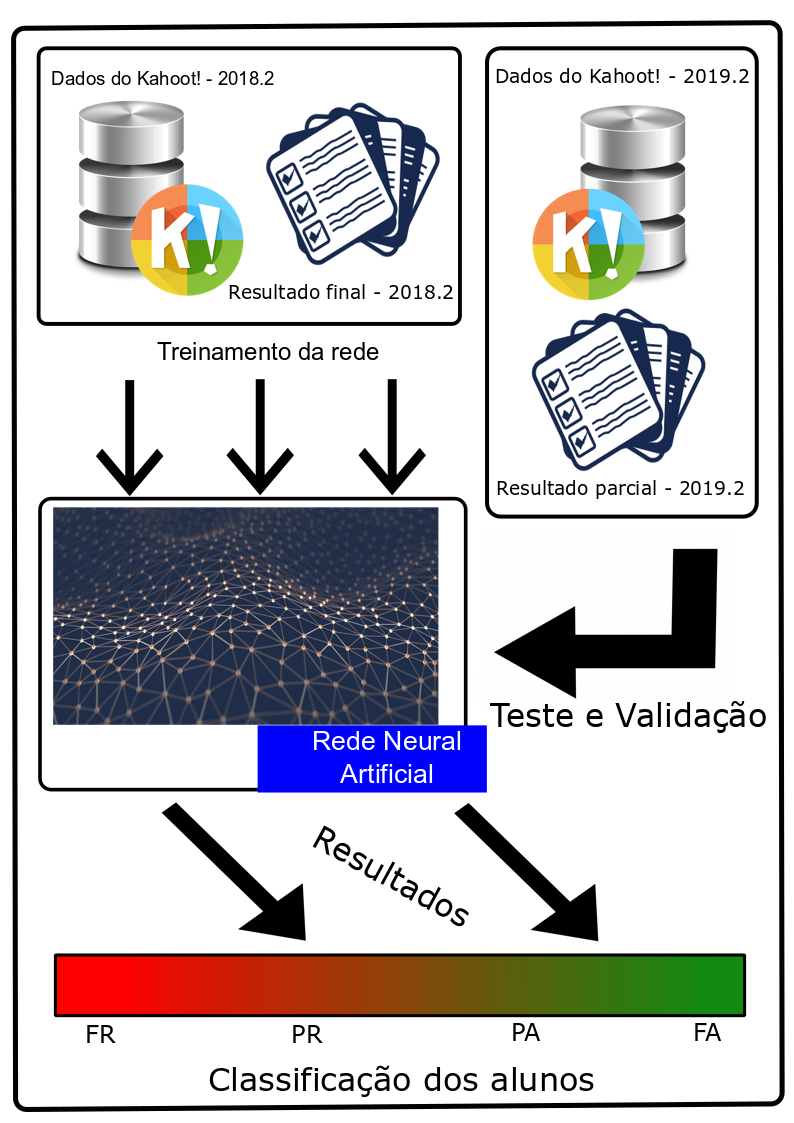
\includegraphics[width=0.9\textwidth]{Modelo_Projeto_Pesquisa_UFG_REJ_BCC/ProcessoMetodologico.png}
    \caption{Diagrama esquemático dos processos do projeto de pesquisa}
    \label{fig:my_label}
\end{figure}

\subsection{Coleta de Dados}
Para este projeto de pesquisa, serão adotadas 4 fontes de dados. Esses dados coletados darão suporte para proposições que serão feitas para solucionar o problema. As quatro fontes de dados que serão usadas são: as respostas do Kahoot! de 2018.2, os resultados finais do processo de avaliação somativa de 2018.2, as respostas do Kahoot! de 2019.2 e os resultados parciais de 2019.2, as quatro na disciplina de Interface Humano-Computador.

\subsubsection{Respostas ao Kahoot!}
O Kahoot! é uma plataforma de GBL e foi descrita melhor na \autoref{sec:Kahoot!}. Na disciplina de Interface Humano-Computador, ela foi utilizada em 2018.2 e será utilizada em 2019.2 novamente. O Kahoot! tem um caráter fortemente formativo, sendo aplicado ao final de cada aula, com questões elaboradas pelo professor que abordem assuntos que foram ministrados na aula. 

As perguntas são de múltipla-escolha, tendo entre duas e cinco alternativas de respostas para o aluno. Neste projeto de pesquisa, serão usados os dados provenientes de respostas dadas pelos alunos aos questionários aplicados nas turmas de 2018.2 e 2019.2 da disciplina de Interface Humano-Computador da UFG, localizada em Jataí, sudoeste goiano.

Na \autoref{fig:kahoot} é apresentado um \textit{Screenshot} de um exemplo de pergunta no Kahoot!

\begin{figure}
    \centering
    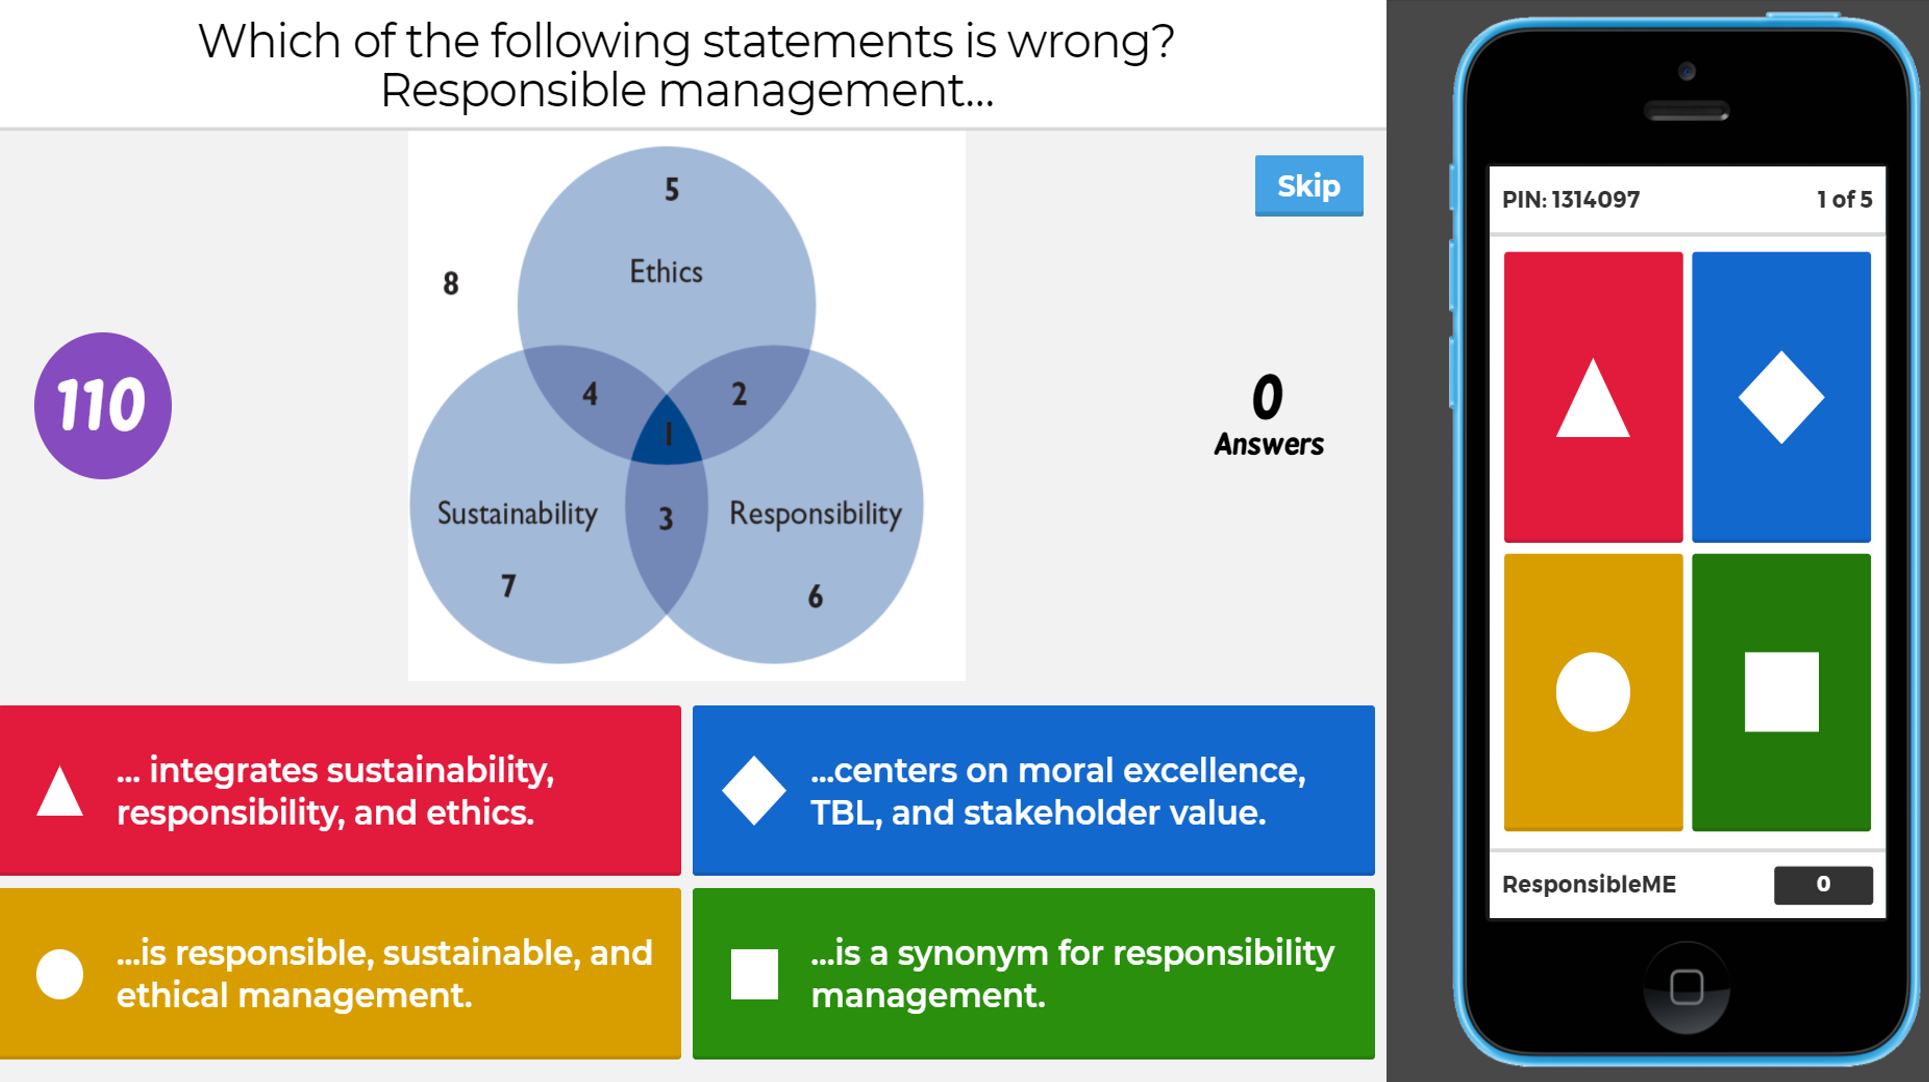
\includegraphics[width=0.9\textwidth]{Modelo_Projeto_Pesquisa_UFG_REJ_BCC/KahootScreenshot.png}
    \caption{Exemplo de uma ``Kahoot!''}
    \label{fig:kahoot}
\end{figure}

\subsubsection{Resultados parciais e finais da Avaliação Somativa}

O processo de Avaliação Somativa foi descrito na \autoref{sec:AvaSom}. O Kahoot! além de caráter formativo, ele também tem, ainda que pouco, caráter somativo. Além disso, serão utilizadas os resultados parciais e finais da disciplina de IHC para a analise dos resultados do projeto.

Na turma de 2018.2, serão usados os resultados finais da Avaliação Somativa. A disciplina já se encerrou, tendo que apenas a posse desses dados para realizar a análise. Já na turma de 2019.2, os resultados da Avaliação Somativa que serão usados são os parciais, consistindo de 2/3 da disciplina já tendo sido realizadas. O motivo desse ocorrido se dá em função do período de obtenção e análise destes, visto que para se ter os resultados finais não haveria tempo hábil para realizar a análise completa destes, tendo assim uma perca. Acredita-se que, com este porção de dados, será suficiente para se ter resultados significativos e, assim, apresentar uma contribuição relevante para a comunidade científica.
 
\subsection{Projeto e Implementação da Rede Neural}

O projeto da Rede consiste em pegar um conjunto de dados de entrada, aplicar essa entrada em neurônios, onde esses reajustarão os pesos destas. A rede produz uma saída com a ``previsão'' da rede, aprovado ou reprovado --- sendo depois indicado o grau, fortemente ou provavelmente. O conjunto de entrada da Rede é composto por um vetor onde estará as respostas dadas pelos alunos.

A Rede Neural Artificial será a técnica de aprendizagem de máquina usada por este projeto de pesquisa. A descrição desta foi feita na \autoref{sec:RNA}. Para isso, será projetada uma Rede Neural Artificial, adotando uma arquitetura de rede especifica.

A implementação da rede será feita na linguagem de programação \textit{Python}, que é uma linguagem interpretada, de \textit{script}, imperativa, orientada a objetos, funcional, de tipagem dinâmica e forte. Python é uma das opções mais comuns, quando se trata de Inteligência Artificial, talvez a que tenha mais biblioteca para Aprendizado de Máquina e Análise de Dados.

Uma destas bibliotecas é a TensorFlow, que é de código-aberto. É com ela que será criada e treinada a Rede Neural proposta por esta pesquisa. Essa biblioteca consiste em detectar e decifrar padrões e correlações, análogo à maneira com que o seres-humanos aprendem e raciocinam.

\subsection{Treinamento da Rede Neural}

Como dito, o treinamento da Rede Neural será feito com a biblioteca TensorFlow na linguagem Python. Os dados usados para esse treinamento da rede seram os dados de 2018.2 e 2019.2 de IHC. O projeto consiste em dividir as resposta pelo período em que elas foram aplicadas, sendo estes em 3 subdivisões.

A primeira rede será a rede com as entradas de dados dos primeiros 15 dias de aula, sendo estas entradas as respostas dadas nesse período às questões do Kahoot!, a segunda divisão será feita da mesma forma, porém as entradas serão as respostas dos primeiros 30 dias de aula. E, por fim, a última rede consistirá das respostas dadas nos primeiros 60 dias de aula.

Nas figuras \ref{fig:rede01}, \ref{fig:rede02} e \ref{fig:rede03}, estão ilustradas como serão feitas as redes, com os conjuntos de entradas. 

\begin{figure}
    \centering
    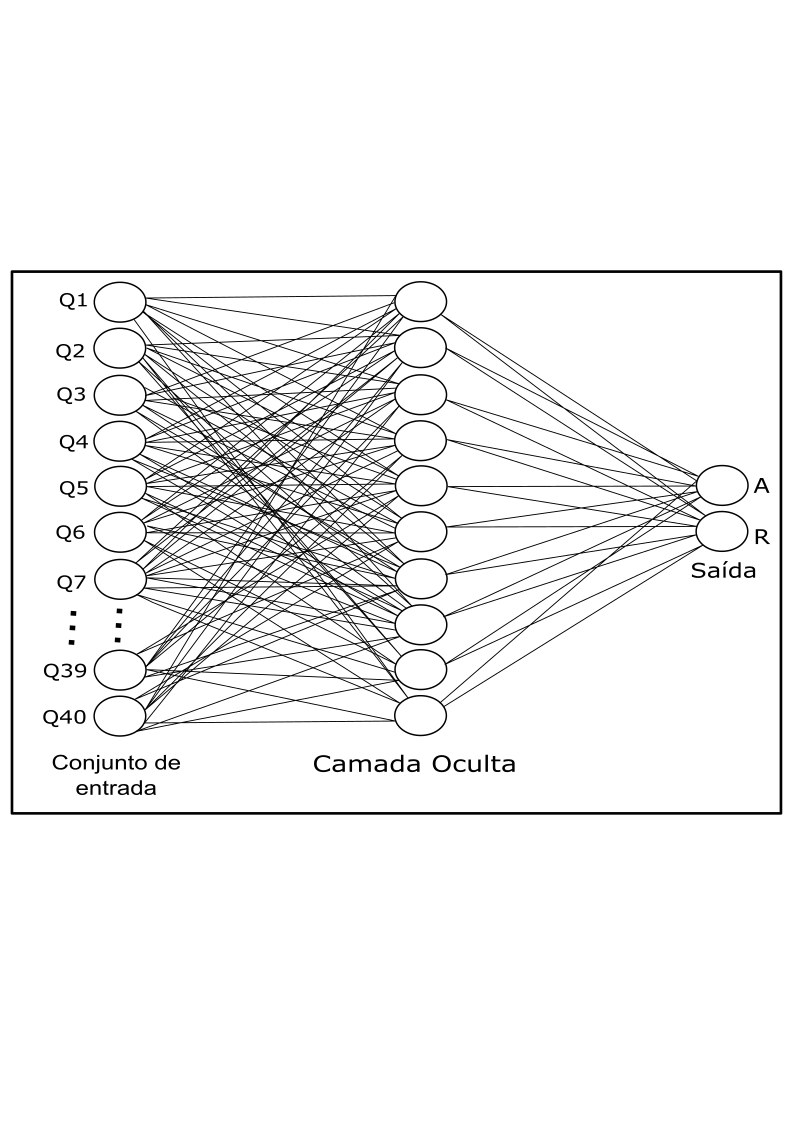
\includegraphics[width=0.9\textwidth]{Modelo_Projeto_Pesquisa_UFG_REJ_BCC/rede01_15.png}
    \caption{Rede 01 - 15 dias de respostas}
    \label{fig:rede01}
\end{figure}

\begin{figure}
    \centering
    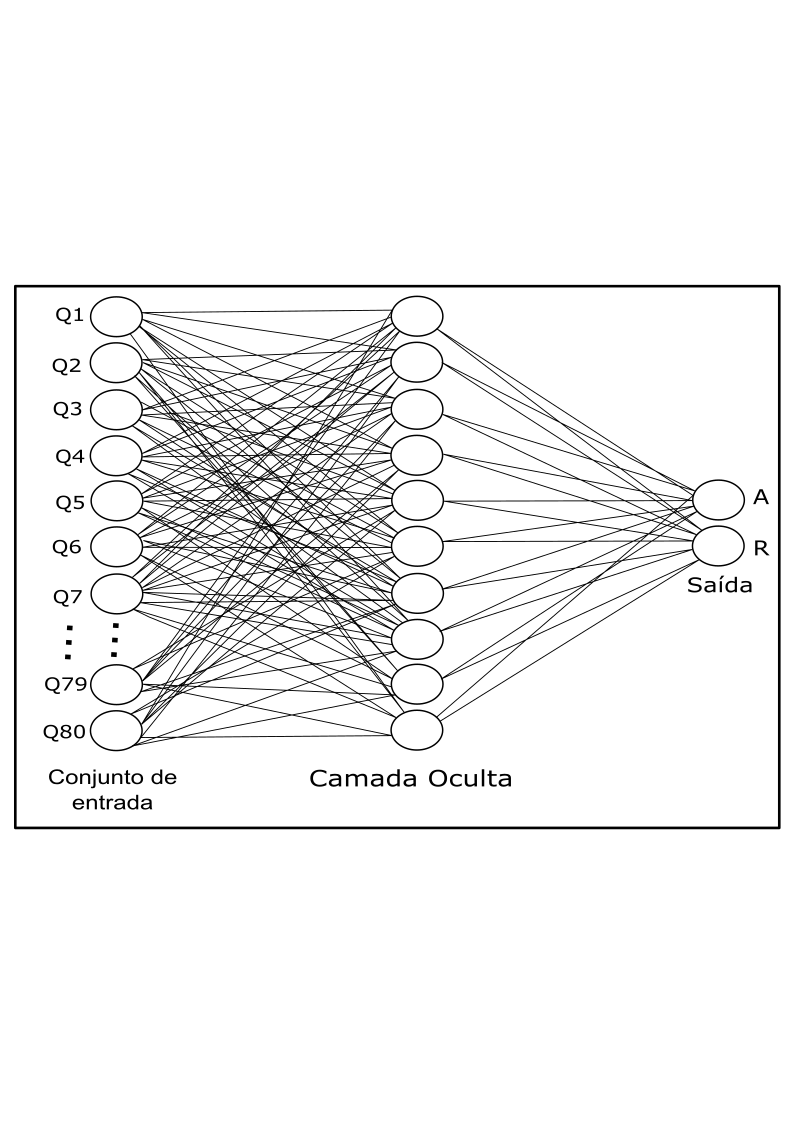
\includegraphics[width=0.9\textwidth]{Modelo_Projeto_Pesquisa_UFG_REJ_BCC/rede02_30.png}
    \caption{Rede 02 - 30 dias de respostas}
    \label{fig:rede02}
\end{figure}

\begin{figure}
    \centering
    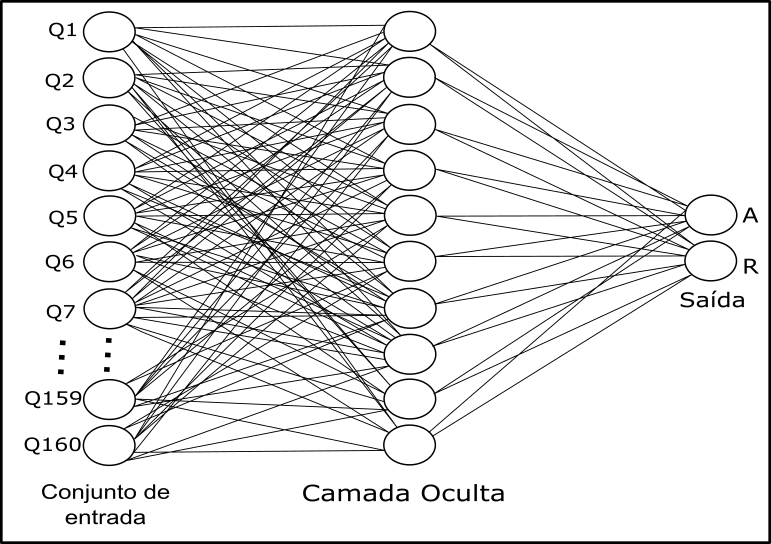
\includegraphics[width=0.9\textwidth]{Modelo_Projeto_Pesquisa_UFG_REJ_BCC/rede03_60.png}
    \caption{Rede 03 - 60 dias de respostas}
    \label{fig:rede03}
\end{figure}

\subsection{Teste e Validação}

O teste e a validação serão feitos nas semanas subsequentes às estabelecidas para o treinamento, com as redes já com os ``neurônios'' com seu respectivo peso, feito através do processo de treino da rede. Ao fazer o teste e a validação, os alunos serão classificados em 4 grupos, que apresentará o grau de risco e a situação dos alunos frente às previsões realizadas pela rede.

\subsection{Classificação dos alunos}
Após a análise ser feita pela Rede, o conjunto de saída apontará o aluno para que este integre um entre quatro grupos que serão estabelecidos. Os grupos seriam definidos como: Fortemente Reprovados (FR), Provavelmente Reprovados (PR), Provavelmente Aprovados (PA) e Fortemente Aprovados (FA). Esses níveis dizem respeito ao quão o aluno está propenso à reprovar. Pensando em um plano cartesiano, seria como se no eixo das abcissas fosse posto esses níveis classificatórios. Nessa analogia, quanto mais à esquerda o aluno fosse classificado, maior seria a chance do aluno ser reprovado na disciplina, quanto mais à direita o aluno fosse classificado, maior seria a chance desse aluno ser aprovado.

A questão que aparece ao se fazer essa classificação é a seguinte: ``Um aluno não pode ser classificado de forma errada?''. Sim, ele pode, e isso é descrito por quatro conceitos (ver \autoref{fig:Venn} importantes de serem definidos neste projeto de pesquisa, que são:

\begin{itemize}
    \item \textbf{Falsos-negativos (FN)}: Com os resultados alcançados pela rede, alunos podem ser classificados como se não estivessem no grupo de risco de reprovação, mas acabam reprovando. São os chamados falsos-negativos.
    \item \textbf{Falsos-positivos (FP)}: Os alunos podem ainda ser classificados como alunos em situação de risco de reprovação, mas ao final da disciplina alguns desses alunos serem aprovados, constatando assim os chamados Falsos-positivos.
    \item \textbf{Verdadeiros-negativos (VN)}: Os alunos classificados como não pertencentes ao grupo de risco de reprovação e que acabam aprovados, sendo assim corretamente classificados previamente, são denominados Verdadeiros-negativos.
    \item \textbf{Verdadeiros-positivos (VP)}: Já os alunos que são classificados como alunos em situação de risco de reprovação e, ao final da disciplina, acabam realmente reprovando, são chamados de Verdadeiros-positivos.
\end{itemize}

\begin{figure}
    \centering
    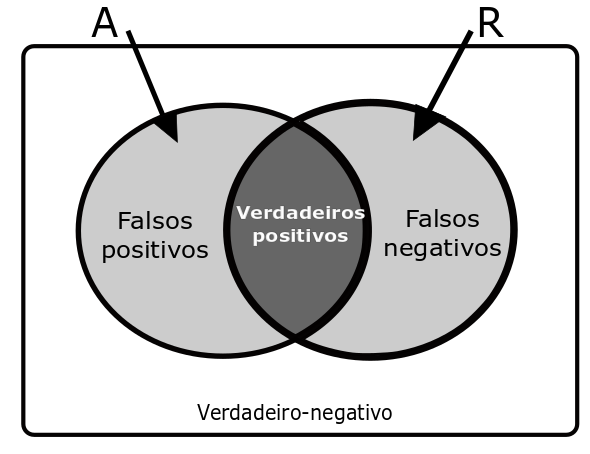
\includegraphics[width=0.9\textwidth]{Modelo_Projeto_Pesquisa_UFG_REJ_BCC/DiagramaVenn.png}
    \caption{Diagrama de Venn para Falsos/verdadeiros negativos e positivos}
    \label{fig:Venn}
\end{figure}

\subsection{Análise dos Resultados}
\label{ss:analise}
Após a produção dos resultados e e classificação da situação dos alunos, o passo seguinte do projeto de pesquisa é analisar os resultados para saber se estes foram satisfatório e estão de acordo com o esperado. Para isso serão usados como métrica os índices de Precisão, Acurácia e Cobertura (\textit{Recall}). As formalizações propostas em outras literaturas para essas três métricas são as seguintes:


$Acurácia = \frac{VP+VN}{VP+VN+FP+FN}*100$

$Precisão = \frac{VP}{VP+FP}*100$

$\textit{Recall} = \frac{VP}{VP+FN}*100$

\section{Estudo de caso}
\label{sec:estudo}
Um estudo de caso é uma investigação empírica que investiga um fenômeno contemporâneo dentro de seu contexto da vida real, especialmente quando os limites entre o fenômeno e o contexto não estão claramente definidos \cite{yin2001planejamento}. Esta investigação enfrenta uma situação tecnicamente única em que haverá muito mais variáveis de interesse do que fonte de dados, e, como resultado, (1) baseia-se em fontes de evidências, com os dados precisando assimilar-se a trabalhos correlatos, e, como outro resultado, (2)beneficia-se do desenvolvimento prévio de proposições teóricas para conduzir a coleta e análise de dados.

\subsection{Descrição do estudo de caso}
Este é um estudo de caso único holístico, utilizando uma estratégia exploratória. A justificativa deste estudo reside no caso revelador que é o uso de RNA na predição de desempenho acadêmico dos alunos em Educação de Computação no Brasil. Os estudos do levantamento bibliográfico concentram-se principalmente em países da América do Norte, Europa e Oceania, como descrito no \autoref{sec:TR}.
Segundo \citeonline{yin2001planejamento}, um estudo de caso contém, em especial, cinco componentes importantes de um projeto de pesquisa que serão descritos a seguir.

%\subsection{Questões do estudo}
Para nortear este estudo de caso, a questão principal levantada foi \textbf{Q1: ``Quais são os resultados ao se utilizar a RNA na previsão de alunos em situação de risco de reprovação em Educação de Computação no contexto Brasileiro?''}

%\subsection{Proposições} \label{sec:HS}
As seguintes proposições foram estabelecidas a fim de serem investigadas. A Proposição 1 \textbf{(P1): ``A precisão da RNA alcançou um nível satisfatório.''}, Proposição 2 \textbf{(P2): ``A acurácia da RNA teve um desempenho satisfatório''} e Proposição 3 \textbf{(P3): ``A cobertura (\textit{Recall}) atingiu um nível satisfatório''}.

\subsection{Unidade de análise, Coleta de Dados}
A unidade de análise do estudo é a turma de 2019.2 da disciplina de Interface Humano-Computador do Bacharelado em Ciência da Computação da Universidade Federal de Jataí, localizada no sudoeste goiano.

A coleta dos dados terá quatro fontes: as respostas dos alunos no Kahoot! de 2018.2 (F1), o resultado final do processo de avaliação somativa dos alunos da turma de 2018.2 (F2), as respostas ao Kahoot! de 2019.2 (F3) e o resultado parcial da avaliação formativa dos alunos da turma de 2019.2 (F4). As duas turmas são da disciplina de Interface Humano-Computador. 

As respostas são dadas pelos alunos, no final de cada aulas, às perguntas elaboradas pelo professor que ministra a disciplina, através da ferramenta de tecnologia educacional, ``Kahoot!'', que foi descrita na seção \ref{sec:Kahoot!} e os resultados parciais e finais no processo de avaliação somativa - aprovado ou reprovado - obtidos por esses alunos.

Ao final da disciplina e do processo de avaliação somativa, os alunos alcançam certo resultado - aprovado ou reprovado - que será um dos dados que formará o conjunto que será analisado.

\subsection{Análise dos Dados}
Para demonstrar a ligação entre os dados coletados e as proposições estabelecidas, serão adotadas três métricas, os resultados de \textbf{precisão}, \textbf{Acurácia} e Cobertura (\textit{Recall} obtidos por trabalhos correlatos. Os dados coletados servirão como suporte para a proposição através da métrica adotada. Se os resultados alcançados forem próximos às métricas, podemos dizer que a previsão feita pela RNA atingiu um nível satisfatório. Mais detalhes serão descritos a seguir. Para melhor compreensão, os conceitos de Acurácia e Precisão são importantes de serem explicados e diferenciados e serão na \autoref{dif}. As fórmulas que os descrevem já foram explicitadas na \autoref{ss:analise}.

As métricas usadas serão usadas como suporte para dizer se os resultados alcançados neste projeto satisfizeram as proposições estabelecidas, ou seja, os níveis alcançados foram satisfatórios. Para definir os valores estabelecidos, tomaremos como base os valores obtidos para os atributos de métrica descritos, evidenciando resultados concretos já alcançados. Os trabalhos em questão serão os Trabalhos Relacionados da\autoref{sec:TR}, onde se alcançaram níveis próximos ao que será estabelecido para este, que terá uma margem de consideração. Formalmente, podemos dizer que as métricas que servirão de base, serão:

$Cobertura = \left \{ x | x >= 70\% \right \}$

$Precisão = \left \{ y | y >= 75\% \right \}$

$Recall = \left \{ z | z >= n\% \right \}$
\subsubsection{Diferença entre Precisão e Acurácia} \label{dif}

\textbf{Precisão} se define como a proximidade entre os valores obtidos pela repetição do processo de mensuração. Quanto menor é a diferença destes valores, melhor é a precisão. \textbf{Acurácia} se define como a proximidade da medida em relação ao verdadeiro valor, um valor definido, que se deseja obter. Quanto mais próximo do valor real, melhor é a acurácia. A \autoref{fig:PrecAcur} esclarece isso de maneira bem didática.

\begin{figure}
    \centering
    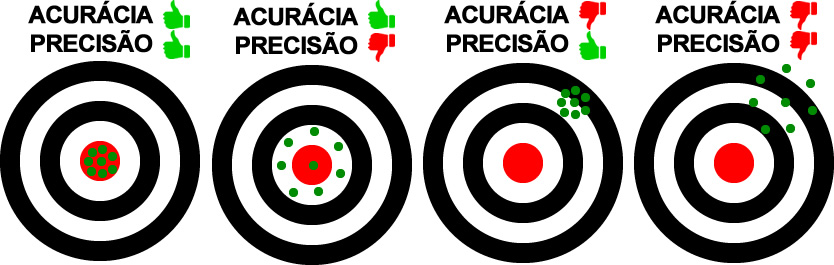
\includegraphics[width=0.9\textwidth]{Modelo_Projeto_Pesquisa_UFG_REJ_BCC/PrecisaoAcuracia.jpg}
    \caption{Diferença entre Acurácia e Precisão}
    \label{fig:PrecAcur}
\end{figure}

%\footnote[4]{Figura disponível em: }

\section{Classificação da pesquisa}
\label{sec:classif}
A classificação desse projeto de pesquisa pode ser feito em termos de gêneros da mesma. Estes gêneros dizem respeito à natureza, os objetivos, os procedimentos, o objeto e à forma de abordagem desta.

\begin{comment}

\subsection{Tipo de Pesquisa}
Essa pesquisa apresenta um \textbf{Estudo de Caso}. Ele será realizadona turma de 2019.2 da disciplina de Interface Humano-Computador, na Universidade Federal de Goias (UFJ/Regional Jatai). Um estudo de caso é uma investigação empírica que investiga um fenômeno contemporâneo dentro de seu contexto da vida real, especialmente quando os limites entre 0 fenômeno e o contexto não estão claramente definidos. \cite{yin2001planejamento}

\subsection{Universo, População e Amostragem/Unidade Local de Análise}
Nesta pesquisa serão envolvidos alunos do curso de Ciência da Computação da Universidade Federal de Goias/Jatai, tendo a população da pesquisa de 162 alunos. E como amostragem, serão usados dados da turma de IHC-2019.2, com aproximadamente 20 alunos {\color{red}[Turma ainda não aberta. Baseando nas últimas duas turmas, média de 20 alunos matriculados]}.

\subsection{Coleta de Dados}
A coleta dos dados - respostas dos alunos às perguntas elaboradas pelo professor que ministra a disciplina - será feita através da ferramenta de tecnologia educacional, ``Kahoot!'', que foi descrita na seção \ref{sec:Kahoot!}

\subsection{Análise e Interpretação dos Resultados/Critérios de Análise}
Como esta se trata de uma pesquisa quantitativa, será usada estatística inferencial para realizar a análise dos dados coletados e dos resultados obtidos.
{\color{red}MELHORAR}

\end{comment}

\subsection{Gêneros de Pesquisa}
\subsubsection{Quanto à natureza}
Empírica, pois a pesquisa dedica-se recolher dados diretamente da realidade do objeto de estudo, mensurar a realidade, formular observações e propor transformações do mesmo enquanto objeto de investigação, mas não intervem de forma concreta no ambiente durante o trajeto da pesquisa.

\subsubsection{Quanto aos objetivos}
Pesquisa exploratória: Apesar de haverem pesquisas em relação à métodos para a predição dos resultados do processo de avaliação somativa --- aprovado ou reprovado ---, há a necessidade de se relatar casos no Brasil, que ocorram experimentos da aplicação desses métodos no processo de avaliação de aprendizagem, identificando alunos em situação de risco.

\subsubsection{Quanto aos procedimentos}
Pesquisa de Campo: Todos os procedimentos que serão usados nesta pesquisa serão derivados de coletas de dados realizadas em fontes diretas. Desta forma, esta pesquisa quantos aos procedimentos é de campo, pois baseia-se em dados coletados no local da ocorrência dos fatos.

\subsubsection{Quanto ao objeto}
Pesquisa de campo: O principal objeto desta pesquisa é justamente a identificação prévia de alunos em risco de reprovação e o uso de Redes Neurais Artificiais como método preditivo. O conceito sobre o objeto, o problema relacionado ao mesmo, assim como a justificativa, são oriundos de uma coleta de dados realizada em local, tornando esta pesquisa de campo quanto aos objetos.

\subsubsection{Quanto à forma de abordagem}
Pesquisa quantitativa: Serão coletadas as respostas dadas pelos alunos, analisando os dados gerados, com o modelo de Rede Neural criado, e produzindo, assim, uma saída classificada.

\begin{comment}{
%===========================================================================================
{\color{red}[MODELO]

\index{elementos textuais} A metodologia em um Projeto de Pesquisa preocupa-se muito mais com a classificação da pesquisa do que propriamente com a condução e execução do trabalho. Porém, o ideal é apresentar o detalhamento metodológico da pesquisa incluindo aspectos técnicos de execução específicos da área. Desta forma, o leitor ou avaliador poderá ter clareza do que será feito e como será feito. Lembrando que a execução metodológica deve estar alinhada com os objetivos específicos descritos na Introdução. 

\begin{enumerate}
\item
Tipo de Pesquisa: Pode-se fazer pesquisa bibliográfica, documental, experimental, estudo de caso e outros tipos. Na área tecnológica, a maioria dos trabalhos é classificada como experimental (quando há um protótipo desenvolvido) e estudo de caso (se situação problemática é relacionada à uma empresa).

\item
	Universo, População e Amostragem:
Deve-se identificar a população da qual você está retirando a sua amostra. Por exemplo, se sua pesquisa envolve os alunos do curso de Sistemas de Informação, sua população é o número total destes alunos, por exemplo 250 alunos. Se você decide então fazer uma amostragem, digamos de 10\%, então sua amostra para fins de sua pesquisa será de 25 alunos.
\item
	Coleta de Dados:
Deve-se indicar como irá operacionalizar a coleta os dados (questionários, check-lists, entrevistas, etc).
\item
	Análise e Interpretação dos Resultados:
Descreve-se neste item como será a análise dos resultados da pesquisa (se a pesquisa for qualitativa, as respostas podem ser interpretadas global ou individualmente, se a pesquisa for  quantitativa, você provavelmente irá utilizar a estatística descritiva ( média, mediana, moda, desvio padrão, tendência central) ou estatística inferencial (regressão linear bivariada, multivariada, etc).
\item
Os gêneros de pesquisa:
Em outra forma descritiva, a pesquisa também pode ser detalhada em termos de métodos obedecendo a classificação de natureza, objetivos, procedimentos, objeto e abordagem:
\begin{enumerate}
\item	Quanto à natureza
\begin{itemize}
\item Teórica - dita como conceitual, procura rever teorias ou formular novas idéias, parâmetros teórico-doutrinários, conceitos.
Metodológica - destina-se a redimensionar novos procedimentos de investigação, modos inovadores de construir ciência, transformação de metodologias tradicionais, introdução de novas técnicas de se conceber o objeto de estudo.
\item Empírica - dedica-se a mensurar a realidade; considera fatores sociais, políticos e econômicos na análise, em outras palavras, parte de constatações empíricas ou da realidade social para solucionar o problema da pesquisa; além disso, formula observações do real e propõe transformações do mesmo enquanto objeto de investigação.
\item Prática - embora semelhante à empírica, difere-se desta por se voltar a intervenções concretas no ambiente político, jurídico, ou sócio-cultural; transformações durante o trajeto da investigação ou análises que proponham novos rumos para a realidade social são os objetivos desse gênero.
\end{itemize}
\item
	Quanto aos objetivos
\begin{itemize}
\item Pesquisa exploratória
- Proporcionar maior familiaridade com o problema;
Levantamento bibliográfico ou entrevistas;
Pesquisa bibliográfica ou estudo de caso.
\item Pesquisa descritiva
- Fatos são observados, registrados, analisados, classificados e interpretados, sem interferência do pesquisador.
- Uso de técnicas padronizadas de coleta de dados (questionário e observação sistemática).
\item Pesquisa explicativa
- Identifica fatores determinantes para a ocorrência dos fenômenos.
- Ciências naturais – método experimental; ciências sociais – método observacional.
\end{itemize}
\item  Quanto aos procedimentos
\begin{itemize}
\item Pesquisa de campo – observação e coleta de dados diretamente no local da ocorrência dos fatos.
\item Pesquisa de fonte documental – pesquisa bibliográfica e documental.
\end{itemize}

\item
	Quanto ao objeto
\begin{itemize}
\item Pesquisa bibliográfica/documental – elaborada a partir de material já publicado (livros de quaisquer espécies, artigos de periódicos).
Pesquisa de laboratório – pesquisador procura refazer as condições de um fenômeno a ser estudado, para observá-lo sob controle.
\item Pesquisa de campo – pesquisador constrói um modelo da realidade, definindo formas de observá-la, formas de acesso a esse campo, os participantes e o campo da pesquisa.
\end{itemize}

\item
	Quanto à forma de abordagem
\begin{itemize}
\item Pesquisa quantitativa – traduz em números as opiniões e informações para serem classificadas e analisadas. Utilizam-se técnicas estatísticas.

\item Pesquisa qualitativa – é descritiva. As informações obtidas não podem ser quantificáveis. Os dados obtidos são analisados indutivamente. A interpretação dos fenômenos e a atribuição de significados são básicas no processo de pesquisa qualitativa. 
\end{itemize}
\end{enumerate}
\end{enumerate}
}
%===========================================================================================
}\end{comment}

%===== Seção de Metodologia ==============


\chapter{Cronograma}

\index{elementos textuais}
    O cronograma tem por objetivo prever as ações distribuídas de acordo com o tempo previsto de pesquisa. Alinhado com os objetivos específicos e com a metodologia, o cronograma descreva em quais prazos os objetivos específicos serão feitos.

A \autoref{tabela_cronog} apresenta o cronograma de execução da pesquisa. 

\begin{table}[!htb]
\centering
\caption{Cronograma de Atividades}
\label{tabela_cronog}
\begin{tabular}{@{}llll@{}}
\toprule
\textit{Atividades}                    & \textit{Mês}       & \textit{Ano}   \\ \midrule
Revisão literária                      & Agosto             & 2019      \\
Projeto e implementação da Rede Neural & Agosto e Setembro  & 2019      \\
Coleta de Dados - IHC/2018.2           & Agosto             & 2019      \\
Coleta de Dados - IHC/2019.2           & Agosto e Setembro  & 2019      \\
Treinamento da Rede Neural             & Setembro           & 2019      \\
Análise dos resultados obtidos         & Outubro e Novembro & 2019      \\
Submissão para o comitê de ética       & Novembro           & 2019      \\
                                %       &                    &           \\ 
                                \bottomrule
\end{tabular}
\end{table}




% ----------------------------------------------------------
% Capitulo com exemplos de comandos inseridos de arquivo externo 
% ----------------------------------------------------------

\include{abntex2-modelo-include-comandos}

% ---
% Finaliza a parte no bookmark do PDF
% para que se inicie o bookmark na raiz
% e adiciona espaço de parte no Sumário
% ---
\phantompart



% ----------------------------------------------------------
% ELEMENTOS PÓS-TEXTUAIS
% ----------------------------------------------------------
\postextual

% ----------------------------------------------------------
% Referências bibliográficas
% ----------------------------------------------------------
\bibliography{abntex2-modelo-references}

% ----------------------------------------------------------
% Glossário
% ----------------------------------------------------------
%
% Consulte o manual da classe abntex2 para orientações sobre o glossário.
%
%\glossary
% ----------------------------------------------------------
% Apêndices
% ----------------------------------------------------------
% ---
% Inicia os apêndices
% ---
%\begin{apendicesenv}
% Imprime uma página indicando o início dos apêndices
%\partapendices
% ----------------------------------------------------------
%\chapter{Exemplo de um apêndice A}
% ----------------------------------------------------------
% ----------------------------------------------------------
%\chapter{Exemplo de um apêndice B}
% ----------------------------------------------------------
%\end{apendicesenv}
% ---
% ----------------------------------------------------------
% Anexos
% ----------------------------------------------------------
% ---
% Inicia os anexos
% ---
%\begin{anexosenv}
% Imprime uma página indicando o início dos anexos
%\partanexos
% ---
%\chapter{Exemplo de um primeiro anexo}
% ---
% ---
%\chapter{Exemplo de um segundo anexo}
% ---
% ---
%\chapter{Exemplo de um terceiro anexo}
% ---
%\end{anexosenv}
%---------------------------------------------------------------------
% INDICE REMISSIVO
%---------------------------------------------------------------------
\phantompart
\printindex
\end{document}